\documentclass[tikz,border=2mm]{standalone}
\usetikzlibrary{arrows,calc}
\usepackage{anyfontsize}
\newcommand{\jiuhao}{\fontsize{2.55pt}{\baselineskip}\selectfont}
\newcommand{\shihao}{\fontsize{1.2pt}{\baselineskip}\selectfont}
\begin{document}
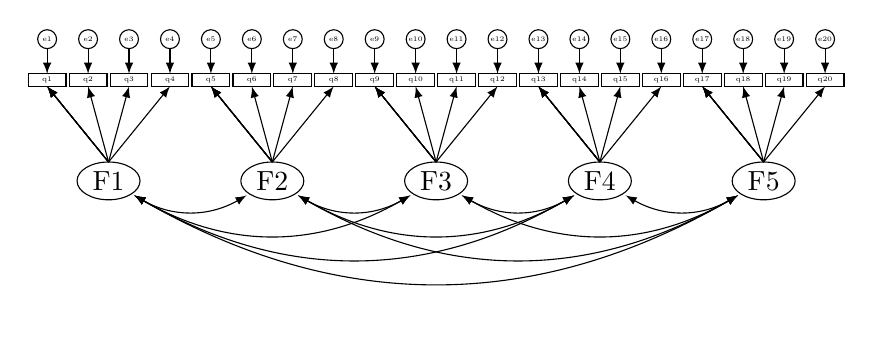
\begin{tikzpicture}[scale=0.4]
%draw circles with adjusted spacing to align with rectangles
\foreach \i in {1,...,20}
\draw (1.3*\i,10.5) circle [radius=0.3] node[font=\jiuhao] {e{\i}};
%draw rectangles with increased width and spacing
\foreach \i in {1,...,20}
    \draw (1.3*\i-0.6,9) rectangle (1.3*\i+0.6,9.4) ;
\foreach \i in {1,...,20}
    \node at (1.3*\i,9.2)[font=\jiuhao]{q{\i}};
%draw ellipses
\draw (3.25,6) ellipse (1 and 0.6);
\draw (8.45,6) ellipse (1 and 0.6);
\draw (13.65,6) ellipse (1 and 0.6);
\draw (18.85,6) ellipse (1 and 0.6);
\draw (24.05,6) ellipse (1 and 0.6);
% draw arrows
\foreach \i in {1,...,20}
\draw [-latex] (1.3*\i,10.2) -- (1.3*\i,9.4);
\foreach \i in {1,...,4}
%\draw [-latex] (3,6.6) -- (\i,9);
\draw [-latex] (3.25,6.6) -- (1.3,9);
\draw [-latex] (3.25,6.6) -- (2.6,9) ;
\draw [-latex] (3.25,6.6) -- (3.9,9) ;
\draw [-latex] (3.25,6.6) -- (5.2,9) ;
\foreach \i in {5,...,8}
% Arrows from the second ellipse to the center of rectangles 5 to 8
\draw [-latex] (8.45,6.6) -- (6.5,9);
\draw [-latex] (8.45,6.6) -- (7.8,9);
\draw [-latex] (8.45,6.6) -- (9.1,9);
\draw [-latex] (8.45,6.6) -- (10.4,9);
\foreach \i in {9,...,12}
% Arrows from the third ellipse to the center of rectangles 9 to 12
\draw [-latex] (13.65,6.6) -- (11.7,9);
\draw [-latex] (13.65,6.6) -- (13.0,9);
\draw [-latex] (13.65,6.6) -- (14.3,9);
\draw [-latex] (13.65,6.6) -- (15.6,9);
\foreach \i in {13,...,16}
% Arrows from the fourth ellipse to the center of rectangles 13 to 16
\draw [-latex] (18.85,6.6) -- (16.9,9);
\draw [-latex] (18.85,6.6) -- (18.2,9);
\draw [-latex] (18.85,6.6) -- (19.5,9);
\draw [-latex] (18.85,6.6) -- (20.8,9);
\foreach \i in {17,...,20}
% Arrows from the fifth ellipse to the center of rectangles 17 to 20
\draw [-latex] (24.05,6.6) -- (22.1,9);
\draw [-latex] (24.05,6.6) -- (23.4,9);
\draw [-latex] (24.05,6.6) -- (24.7,9);
\draw [-latex] (24.05,6.6) -- (26.0,9);
\node[above] (a) at (3.25,5.4) {F1};
\node[above] (b) at (8.45,5.4) {F2};
\node [above](c) at (13.65,5.4) {F3};
\node [above](d) at (18.85,5.4) {F4};
\node[above] (e) at (24.05,5.4) {F5};
%\draw[<->,-latex] (a) -- (b);
\draw[<->,>=latex,bend right]  (a) to (b);
\draw[<->,>=latex,bend right]  (b) to (c);
\draw[<->,>=latex,bend right]  (c) to (d);
\draw[<->,>=latex,bend right]  (d) to (e);
\draw[<->,>=latex,bend right]  (a) to (c);
\draw[<->,>=latex,bend right]  (a) to (d);
\draw[<->,>=latex,bend right]  (a) to (e);
\draw[<->,>=latex,bend right]  (b) to (d);
\draw[<->,>=latex,bend right]  (b) to (e);
\draw[<->,>=latex,bend right]  (c) to (e);

\end{tikzpicture}
   \end{document} 
